\section{Decision Tree}
In this section we will discuss the implementation, choice of hyperparameters and results of the \class{DecisionTreeClassifier()}.
A decision tree is a supervised machine learning model that can be used for regressing or classification.
It works by building a tree-like structure, where at each internal node, the algorithm considers all the available features and chooses the split that maximizes the purity of the resulting splits.
This process is repeated until a certain stop condition is reached, such as a maximum depth or no further improvement in purity.
Decision tree classifiers are popular because they are easy to understand and interpret due to their tree-like structure, and they can handle different data types and types of decision boundaries. \\

\begin{figure}[H]
    \centering
    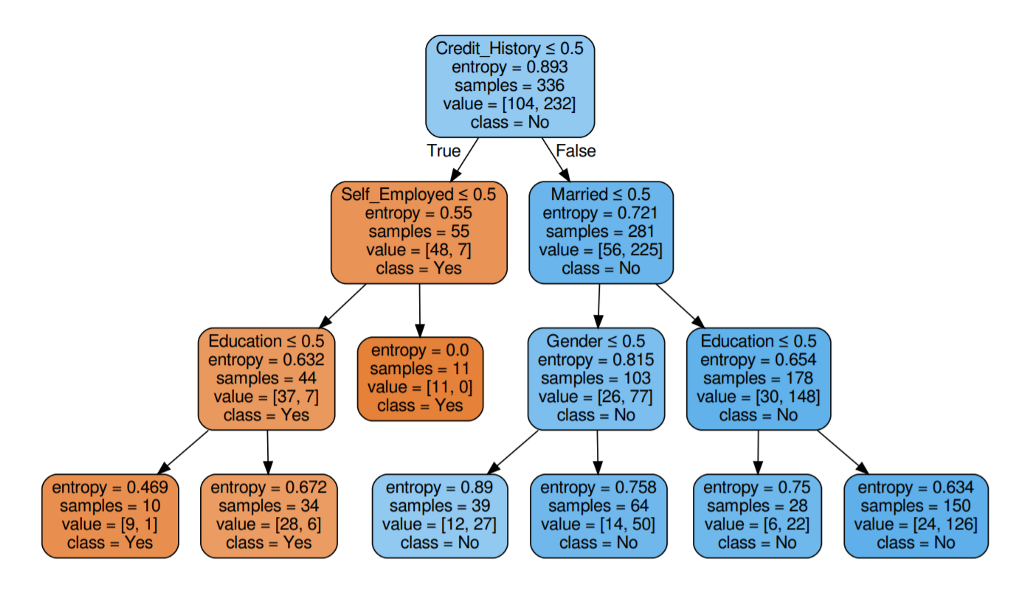
\includegraphics[scale=0.25]{figures_for_report/example_decision_tree}
    \captionsetup{justification=centering,margin=2cm}
    \caption{Simple Decision Tree}
\end{figure}


\subsection{Implementation}
As this project is focused on classification rather than regression a classification tree was implemented.
It was done in Python using two classes:
\begin{enumerate}
    \item \class{Node()}
    \item \class{DecisionTreeClassifier()}
    \end{enumerate}
\vspace{10pt}

\subsubsection{Node}
The \class{Node()} class has the most responsibility of the two.
It holds the data and passes it down the tree constantly splitting itself into more nodes with the \code{_split()} method.
This is done by finding the best split with the \code{_get_best_split()} method based on the impurity measure specified.
The best split refers to the feature and cutoff value that leads to the highest gain in purity in the two resulting nodes.
After finding the best split, it can then create two new nodes, \code{self.left} and \code{self.right} if all split criteria are fulfilled.
The two criteria implemented are \code{max_depth} and \code{min_samples_split} and are discussed further in the \class{DecisionTreeClassifier()} implementation.
This splitting process is what happens recursively in the \code{fit()} method in the \class{DecisionTreeClassifier()}, and is how the tree-structure is build. \\

\subsubsection{DecisionTreeClassifier}
The \class{DecisionTreeClassifier()} class is the classifier interface
which has the \code{fit()} and \code{predict()} methods and some 'less' important
methods \code{get_depth()} and \code{get_n_leaves()}, that can be called after the model has been fitted.
The \code{fit()} method as mentioned earlier simply starts with a root \class{Node()} and calls \code{_split()} recursively.
The \code{predict()} method works by using the sample input to traverse down the tree until a leaf is reached, and predicting the most common class.\\
Our implementation allow for specification of the following 4 parameters.\\
\begin{enumerate}[label=(\roman*)]
    \item \code{max_depth} -- (specify maximum depth to which the tree can grow)
    \item \code{min_samples_split} -- (specify minimum number of samples in a node before it can be split)
    \item \code{criterion} -- (split based on either gini or entropy)
    \item \code{random_state} -- (set random seed for reproducible results)
    \end{enumerate}
\vspace{10pt}

\subsection{Asserting Correctness}
To validate the correctness of our implementation a thorough comparison with the sklearn version was done.
First a comparison of 100 sklearn models and 100 of our models accuracy score was done using the \code{load_digits()} dataset from \code{sklearn.datasets}
This can be seen in Figure 5.\\

\begin{figure}[ht]
    \centering
    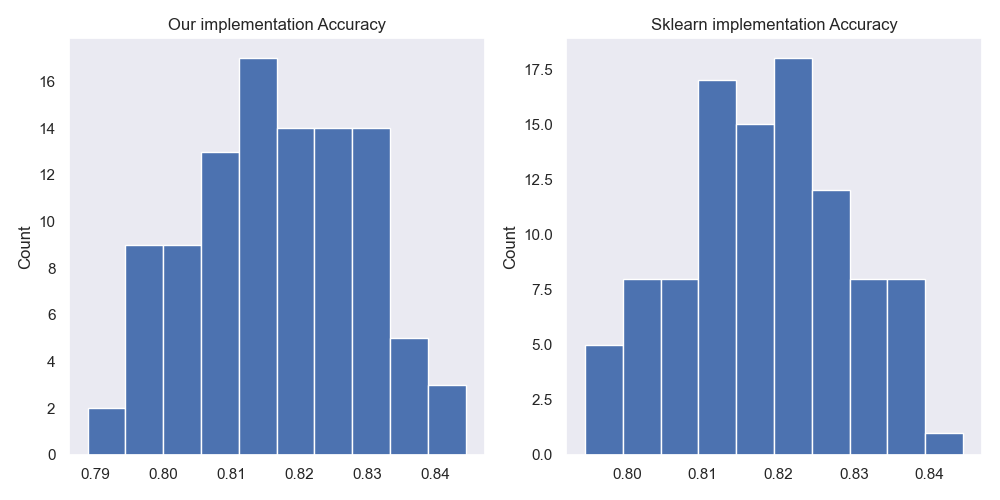
\includegraphics[scale=0.55]{figures_for_report/our_vs_sklearn_accuracy}
    \captionsetup{justification=centering,margin=2cm}
    \caption{Accuracy distribution from 100 models}
\end{figure}

Each decision tree used in Figure 5 is fitted with the default parameters of both the sklearn and our model.
This means that the \code{max_depth} is not restricted and the \code{min_samples_split} is set to 2.
A decision tree has randomness involved in the training process.
This is because if two splits yield the same gain one of them will be chosen at random.
This means the models might perform slightly different in a single test but very similar on average.\\

The resulting tree depths and number of leaves were also compared and showed that the decision trees in both implementations grow to the same
depth and with the same number of leaf nodes.
\\

Lastly a comparison of \textbf{some} of the actual splits (best feature and cutoff) were done to assert correctness and as a sanity check, and
the two implementations also agreed on this.\\

\subsection{Hyperparameters}
A decision tree is very prone to overfitting to the training data.
This is especially the case if the max depth or other early stopping to the growth is not controlled.
This can lead to a  very high training accuracy but might struggle with unseen data.
Another way to control this is using post-pruning where the tree is first grown fully, and then afterwards its size is reduced.
This was not implemented in our model so what was tried instead was to find the optimal \code{max_depth}, to reduce overfitting.
Along with finding an optimal \code{max_depth}, a good combination of \code{max_depth}, \code{min_samples_split} and
\code{criterion} (gini or entropy) was found.
This was done \class{GridSearchCV()} from sklearn, where a range of values for each of the mentioned parameters was searched for.
\class{GridSearchCV()} uses cross-validation, in this case 5-fold, on the training data, and tests all combinations specified in the following parameter grid:

\begin{center} \begin{minipage}{4in}

\begin{itemize}
    \item \code{max_depth}: [None, 5, 7, 9, 11, 12]
    \item \code{min_samples_split}: [2, 4, 8, 10]
    \item \code{criterion}: [gini, entropy] \\
\end{itemize}
            \end{minipage}
\end{center}

This gave the best combination as \code{max_depth=9}, \code{min_samples_split=4}, \code{criterion=gini}.
This combination was then used to train our own implementation and the results will be reported in the next section


\subsection{Results}








\begin{table}[!ht]
\begin{subtable}[c]{0.4\textwidth}
\footnotesize
\centering
\begin{tabular}{ c | c }
 \toprule
 Evaluation Metric & Accuracy Score  \\
 \midrule
 Training Accuracy &  89.83\% \\
 Test Accuracy &79.32\% \\
 \bottomrule
\end{tabular}
\captionsetup{justification=centering,margin=1cm}
\end{subtable}
\begin{subtable}[c]{0.6\textwidth}
\footnotesize
\centering
\begin{tabular}{c | c c r}
Class & Precision & Recall & F1-Score\\
\midrule
T-shirt/Top   &    0.76  &    0.75  &    0.75 \\
Trousers   &    0.97  &    0.92  &    0.95 \\
Pullover   &    0.80  &    0.83  &    0.81\\
Dress   &    0.82  &    0.88  &    0.85\\
Shirt   &    0.61  &    0.60  &    0.60\\
\end{tabular}
\captionsetup{justification=centering,margin=1cm}
\end{subtable}
\caption{Decision Tree Performance Evaluation}
\label{dt_evaluation}
\end{table}\\

The results reported is from our own implementation of the \class{DecisionTreeClassifier()} with the parameters specified earlier.
To reproduce these results the \code{random_state} parameter should be set to 42.

\subsubsection{Discussing Results}







